\chapter{LA REPRESENTATION DE LA DONNEE}

\section{Introduction}
     \vspace{1em}

Envoyer une donnée sur un réseau n’est pas aussi simple que l’on croit.
     \vspace{1em}

 \begin{wrapfigure}{r}{3cm}
\Youtube{https://youtu.be/k-RhgiwKx2M}
\end{wrapfigure}
Il faut faire la différence entre le format utilisé pour stocker des données dans la mémoire de l'ordinateur et celui employé pour l'envoyer à une autre machine. En effet, chaque machine à sa propre représentation souvent liée aux capacités de leur processeur. Cela est surtout vrai pour les nombres. Ils peuvent être stockés sur un nombre de bits plus ou moins important ou peuvent être représentés en mémoire de manière optimisée pour accélérer leur traitement. 

En revanche, la représentation des chaînes de caractères (non accentués) est relativement uniforme car elle se base sur le code ASCII qui est le même pour tous les ordinateurs. Un texte de base est facilement compréhensible par toutes les machines. Une solution serait donc de n'utiliser que des chaînes de caractères. 

     \vspace{1em}

Par exemple, si l’on veut envoyer l'entier ayant pour valeur 123, il existe plusieurs représentations possibles :
\begin{itemize}
\item envoyer une chaîne de caractères ”123” contenant les chiffres du nombre ;
\item envoyer la valeur binaire 1111011.
\end{itemize}

     \vspace{1em}

On voit que juste pour transmettre une simple valeur stockée dans la mémoire d'un ordinateur, il existe plusieurs options et évidemment pour que cette valeur soit interprétée de la bonne façon, il faut que les deux extrémités se soient mises d'accord sur une représentation.

Quand on veut transmettre plusieurs valeurs, c'est-à-dire quand on a des données structurées, d'autres problèmes surviennent.

Par exemple : quelle est la taille des blocs que l’on va transmettre ? Comment indiquer la fin de la transmission ? Pour une chaîne de caractères, comment indiquer qu’elle se termine ? Autre exemple : si l'on veut transmettre "12" puis "3", comment faire pour que l'autre extrémité ne comprenne pas "123" ?

     \vspace{1em}


Pour que la transmission se fasse correctement, il faut que l’émetteur et le récepteur adoptent les mêmes conventions. Quand il s’agit d’un ensemble de données, il faut être capable de les séparer. Avec les tableurs, une première méthode est possible avec la notation \ac{CSV} Comme son nom l’indique, les valeurs sont séparées par des virgules. Les valeurs sont représentées par des chaînes de caractères. Les textes sont différenciés des valeurs numériques, par l’utilisation de guillemets. Ainsi, 123 sera interprété comme un nombre et ”123” comme un texte.

Si cette représentation est adaptée aux tableurs, elle est relativement pauvre car elle ne permet de représenter que des valeurs sur des lignes et des colonnes. Pour les usages du Web, il a fallu trouver un format plus souple permettant de représenter des structures de données complexes. Évidemment, comme rien n'est simple, il en existe plusieurs et les applications échangeant des données devront utiliser le même.

     \vspace{1em}


On voit que l'envoi de la chaîne de caractères ne suffit pas, il faut la formater pour que le récepteur puisse trouver le type de la donnée transmise, qu'un nombre ne soit pas interprété comme une chaîne de caractères, qu'une chaîne de caractères reste une chaîne de caractères même si elle ne contient que des chiffres.   
    \vspace{1em}
   
\section{La \Index{sérialisation}}

Sous ce nom barbare se cache la méthode utilisée pour transmettre 
des données d’un ordinateur à un autre.
Une donnée peut être simple
(un nombre, un texte) ou plus complexe (un tableau, une structure...). 
Elle est stockée dans la mémoire de l'ordinateur suivant une représentation qui lui est propre. Par exemple, la taille des entiers peut varier d'une technologie de processeur à une autre, l'ordre des octets dans un nombre peut aussi être différente (little et big endian). 
Pour des structures complexes comme les tableaux, les éléments peuvent être rangés à différents emplacements de la mémoire. 

La sérialisation consiste à transformer une structure de données en une séquence qui pourra être transmise sur le réseau, stockée dans un fichier ou une base de données. L'opération inverse, consistant à reconstruire localement une structure de données, s'appelle désérialisation. 

Il existe plusieurs formats pour sérialiser les données. Ils peuvent être binaires mais ceux généralement utilisés sont basés sur des chaînes de caractères. En effet, la représentation \ac{ASCII} définissant les caractères de base et codée sur 7 bits est commune à l'ensemble des ordinateurs. L'autre avantage du code ASCII est qu'il est facilement lisible et simplifie la mise au point des programmes.  

Wikipédia donne ce tableau (cf. figure~\vref{fig-ASCII}) des codes \ac{ASCII} datant de 1972 (une éternité en informatique) et recolorisé par nos soins.

\begin{figure}[tbp]
\centerline{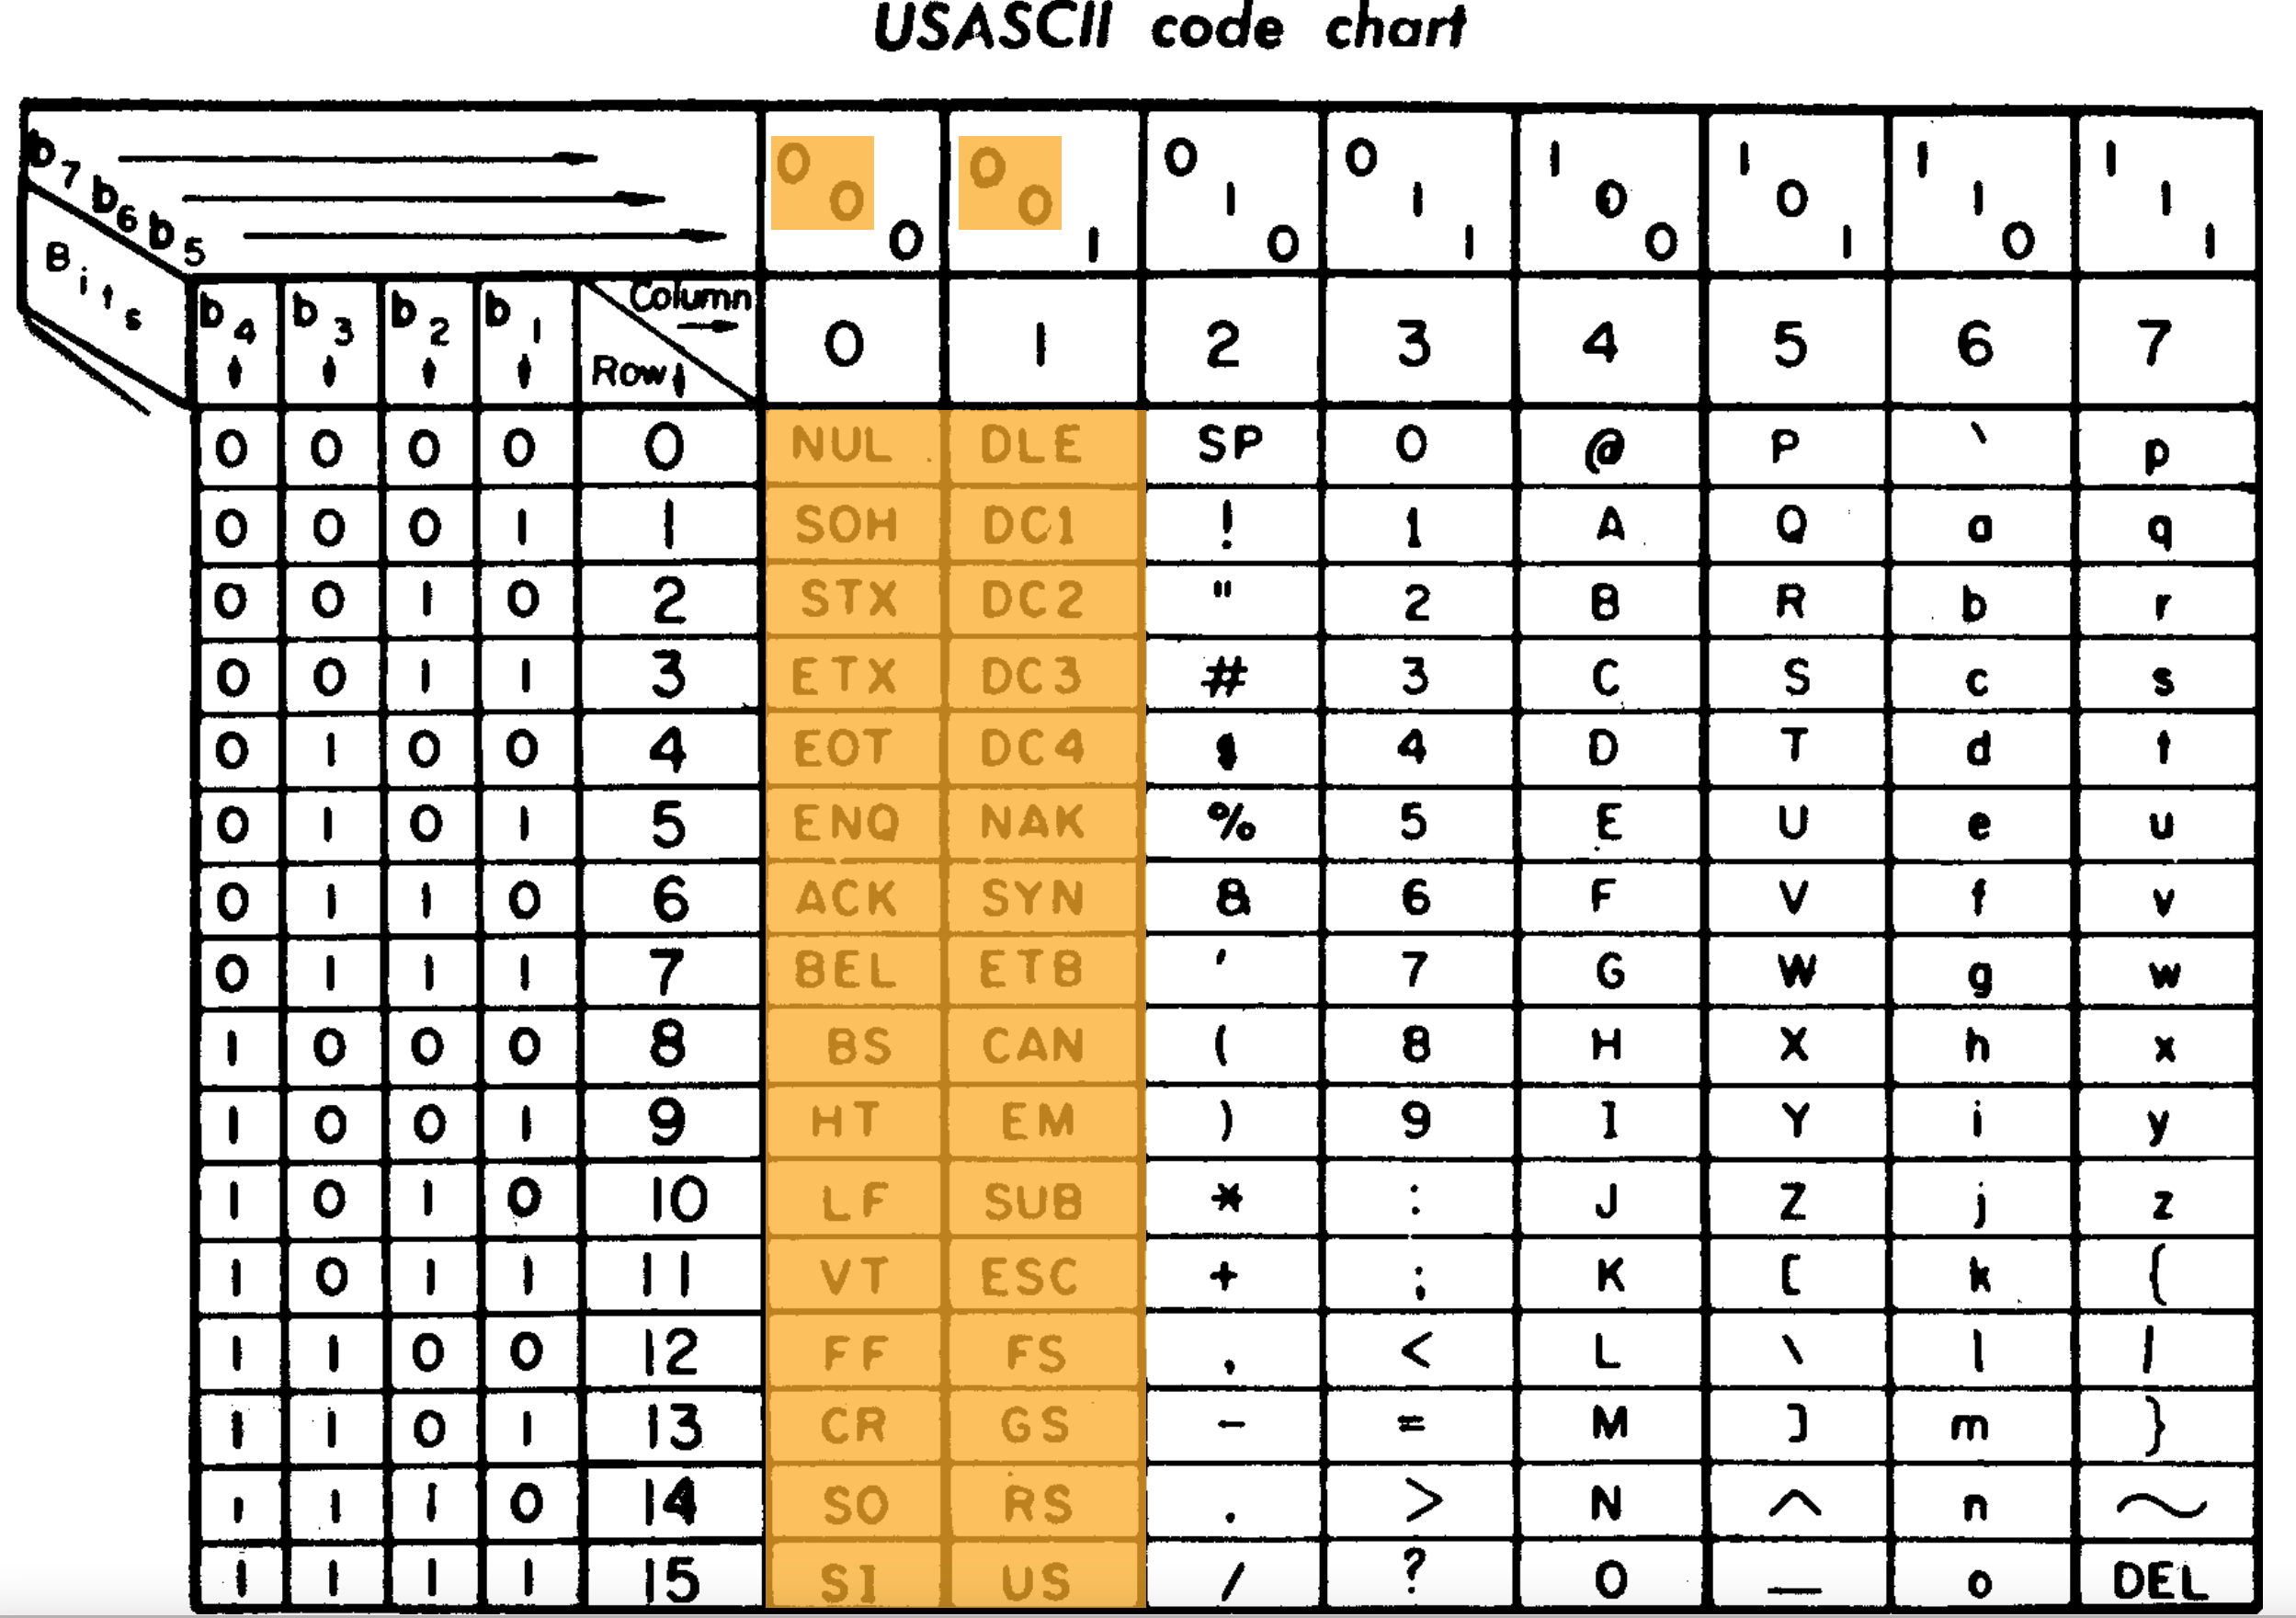
\includegraphics[width=1\columnwidth]{Pictures/Capture20.png}}
\caption{Codage ASCII des caractères}
\label{fig-ASCII}
\end{figure}

Les caractères en orange ne sont pas imprimables. Ils permettent de contrôler la communication des données ou de gérer l'affichage en revenant à la ligne. On les reconnait car la séquence binaire commence par 00X XXXX. On rappelle que le code ASCII est sur 7 bits ; le bit supplémentaire (bit de parité) conduisant à 1 octet était utilisé pour détecter des erreurs de transmission. Les valeurs de 0x30 à 0x39 codent les chiffres de 0 à 9. 

\subsection*{Hexlify}

En Python, il existe le module \Index{binascii} très pratique qui permet de convertir une séquence binaire en une chaîne de caractères ou inversement :
\begin{itemize}
\item \pfunction{binascii}{hexlify} prend un tableau d'octets et le convertit en une chaîne de caractères hexadécimaux plus lisible pour les spécialistes. Cela permet de visualiser n'importe quelle séquence de données. 
\item \pfunction{binascii}{unhexify} fait l'inverse. Il prend une chaîne de caractères et la convertit en un tableau d'octets. Cela peut vous faciliter la programmation car, dans votre code, il est plus facile de manipuler des chaînes de caractères.

\end{itemize}
Dans la suite, nous l'utiliserons pour manipuler des identifiants. Par exemple, ce bout de code illustre l'utilisation de ces fonctions :

\begin{python}
mac = lora.mac()
print ('devEUI: ',  binascii.hexlify(mac))

# create an OTAA authentication parameters
app_eui = binascii.unhexlify('70 B3 D5 7E D0 03 3A E3'.replace(' ',''))

\end{python}

Comme nous le verrons par la suite, a fonction \pfunction{network}{lora.mac()} retourne un tableau d'octets. La fonction \pfunction{binascii}{hexlify} ligne suivante le convertit en chaîne de caractères pour un affichage plus propre. 

Inversement, nous devons affecter une séquence binaire à la variable \texttt{app\_eui}. Nous mettons cette séquence hexadécimale en chaîne de caractères. Les espaces offrent plus de lisibilité. Ils sont retirés par la méthode replace et le résultat est converti en binaire grâce à \pfunction{binascii}{unhexify}

\section{Base64}

Le passage d'une séquence binaire à une chaîne de caractères ASCII en représentant les valeurs conduit à un doublement du volume. Chaque bloc de 4 bits va conduire à produire un octet correspondant au caractère d'un chiffre ou d'une lettre de A à F. Le reste des codes n'est pas utilisé.

Le codage base64 offre un meilleur rendement en utilisant 64 bits pour coder les valeurs. Un dictionnaire fait la correspondance entre 64 valeurs et un caractère ASCII. Cependant, si l'on veut coder 4 octets, soit 32 bits, il faudra 5 blocs de 6 bits, et il y aura deux bits restants. Le symbole = indique que 2 bits sont ajoutés à la fin du codage. Donc, dans notre cas, il faudra ajouter deux symboles = comme le montre la figure ci-dessous :

\begin{figure}[tbp]
\centerline{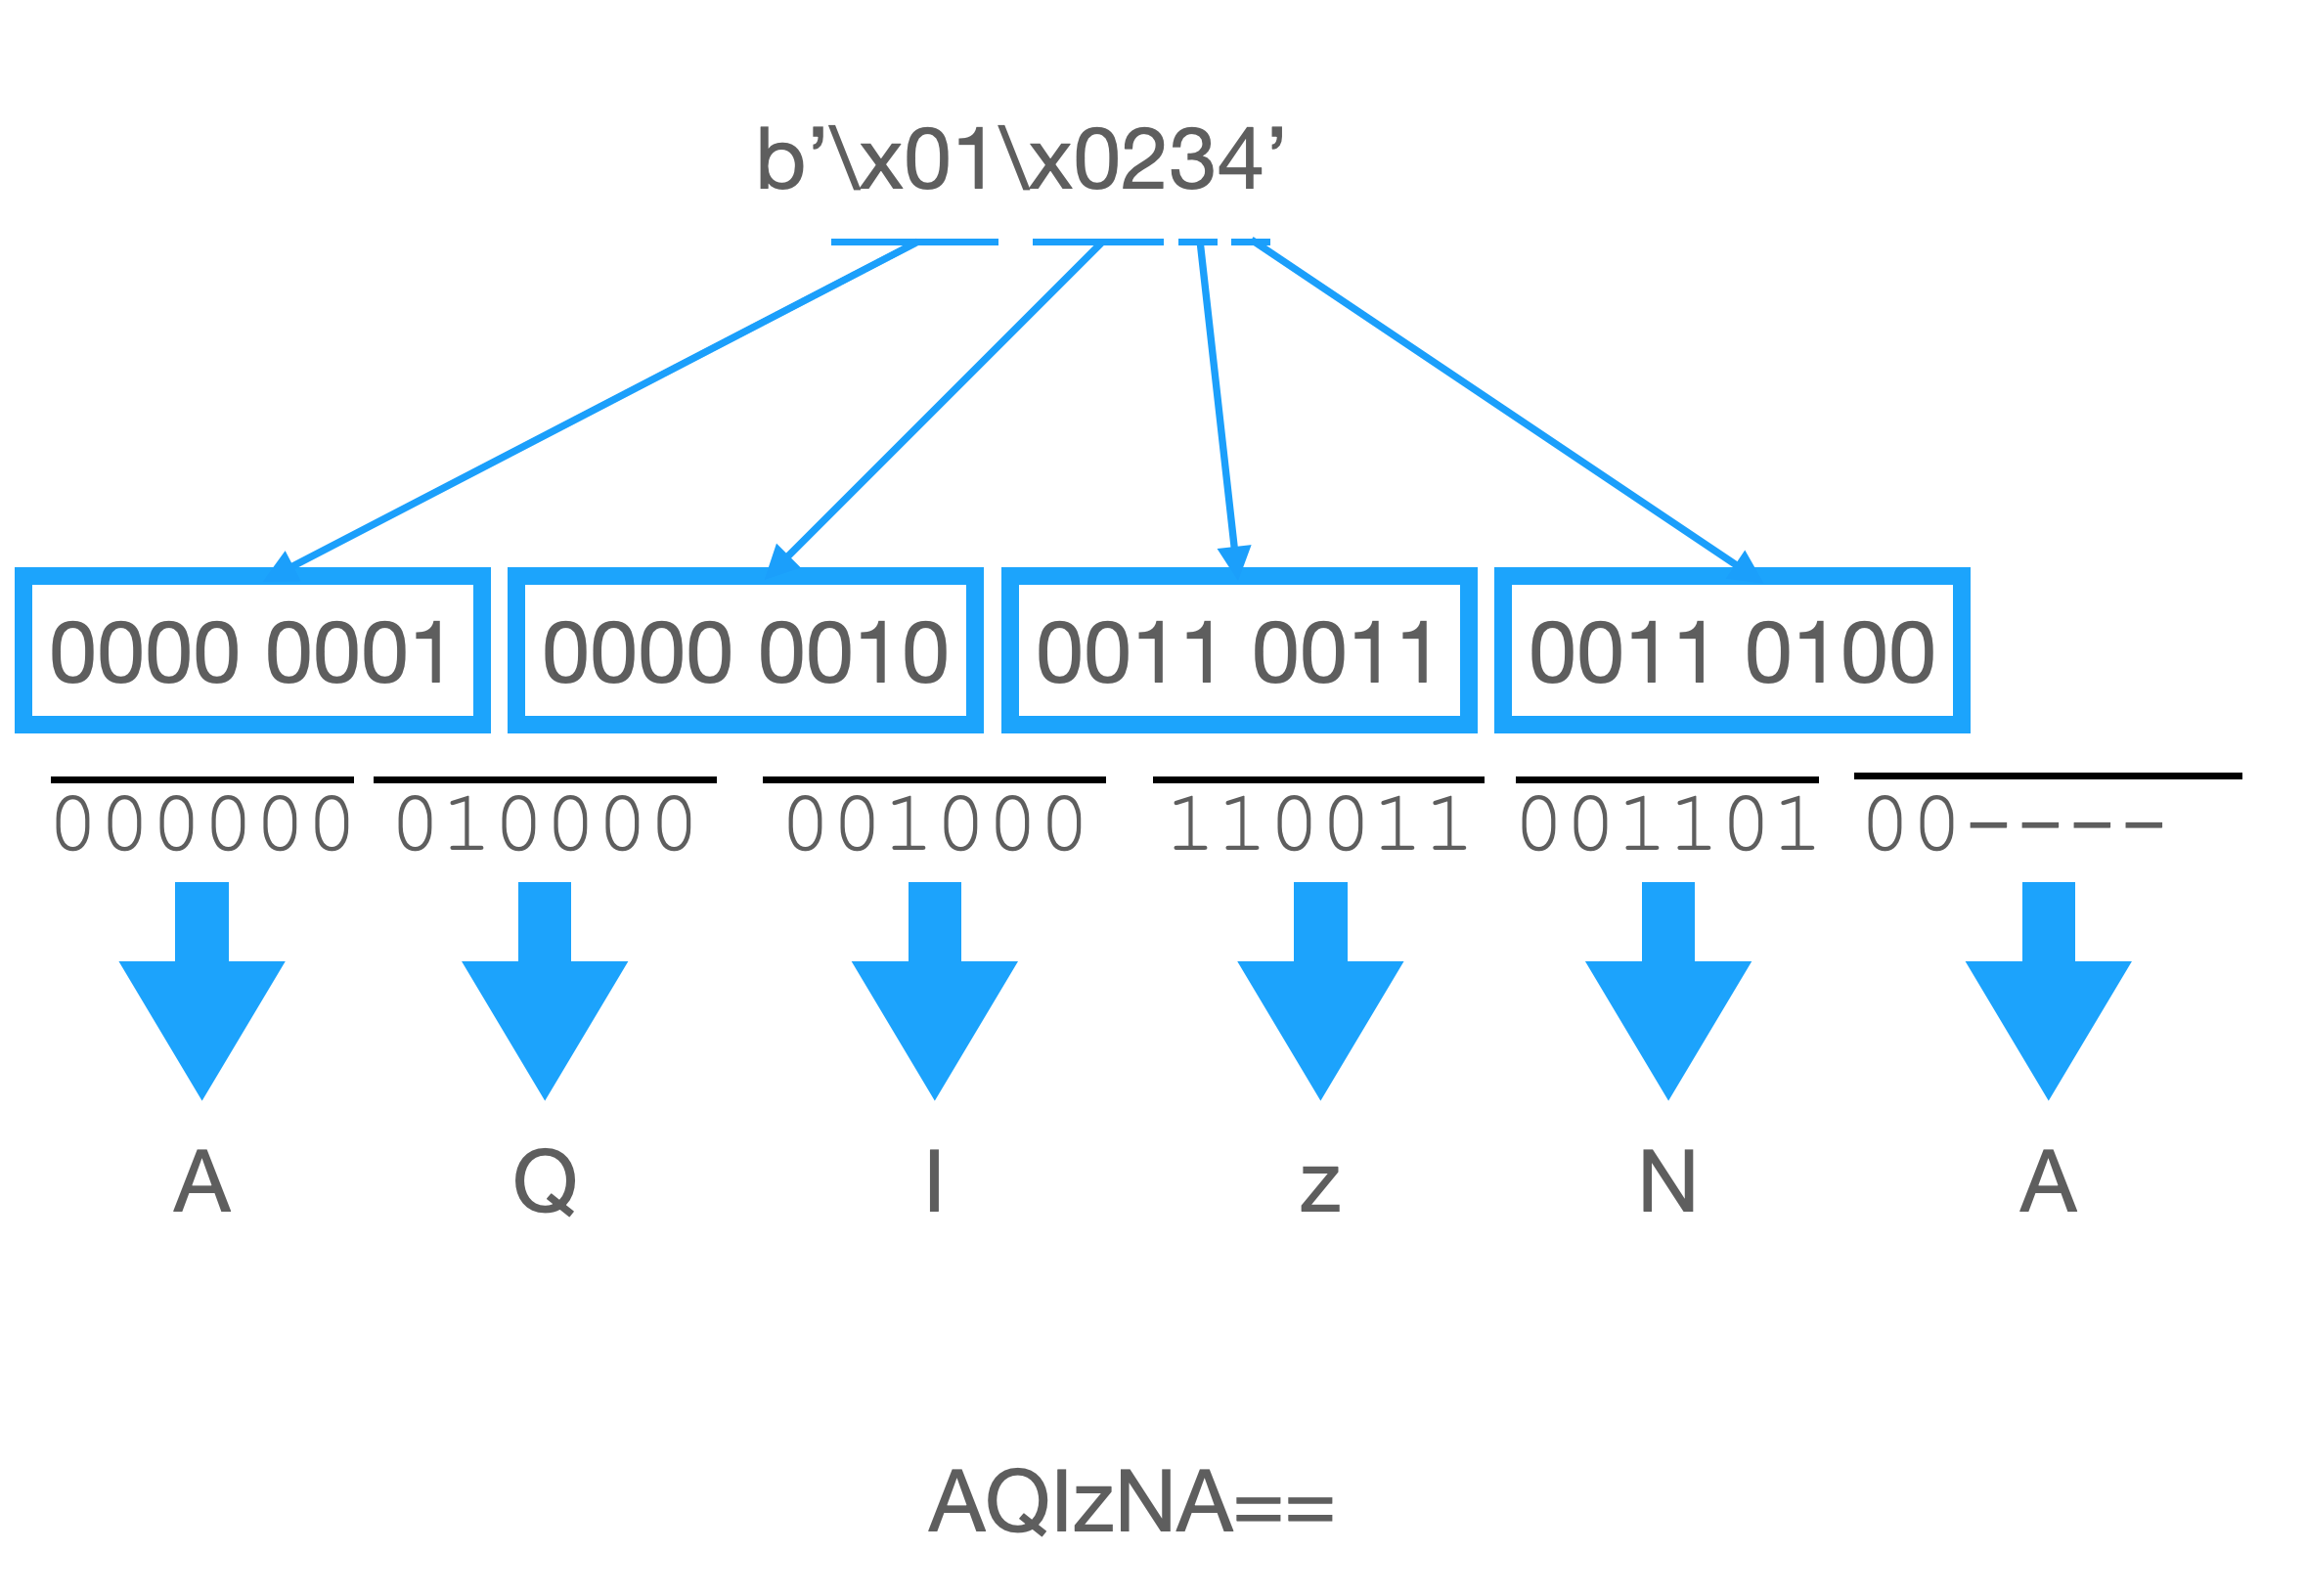
\includegraphics[width=1\columnwidth]{Pictures/Capture21.png}}
\caption{Codage Base64 de données binaires}
\label{fig-base64}
\end{figure}

On notera que pour les petites séquences, ce codage n'est pas meilleur que la transformation de la séquence hexadécimale en chaîne de caractères. Ici, il faut 8 caractères pour coder 4 octets. 

Il existe beaucoup d'outils en ligne pour faire les conversions entre ces différentes représentations, comme le site \url{www.asciitohex.com}.

\subsection*{Python module: base64}

En Python3, le module base64 permet de faire ces conversions.  Ce module est un peu susceptible sur les types de données à utiliser.

\begin{python}[numbers=left,numbersep=5pt]
import base64

val = b"\x01\x0234"
ser = base64.b64encode(val)
print (ser)
print (ser.decode())
ori = base64.b64decode(ser)
print (ori)
\end{python}

qui donne à l’exécution :

\begin{termc}[backgroundcolor=\color{backcolour}]
b'AQIzNA=='
AQIzNA==
b'\x01\x0234'
\end{termc}

À noter que l'utilisation du \texttt{ser.\pfunction{str}{decode}()}, ligne 6, pour transformer une chaîne d'octets en chaîne de caractères, c'est-à-dire supprimer le \texttt{b} du début, peut être utilisé dans certains cas.



\section{HTML}

La sérialisation en chaînes de caractères (par exemple en Python via la commande \pfunction{binascii}{hexlify}) ou en Base64 concerne surtout des données binaires. Mais la donnée peut être aussi structurée, par exemple la page d'un tableur. Il faut donc formater le document pour éviter une fusion des différents champs.


\ac{HTML}, sans entrer dans les détails, définit un format où les champs sont repérés par un balisage.  Une balise de début est un mot clé entre \texttt{<>} et, pour une \Index{balise} de fin, le mot clé est précédé du caractère \texttt{/}. Par exemple, la figure~\vref{fig-HTML} avec le balisage, le premier paragraphe est formaté de cette manière, Dans le MOOC :

\begin{figure}[tbp]
\centerline{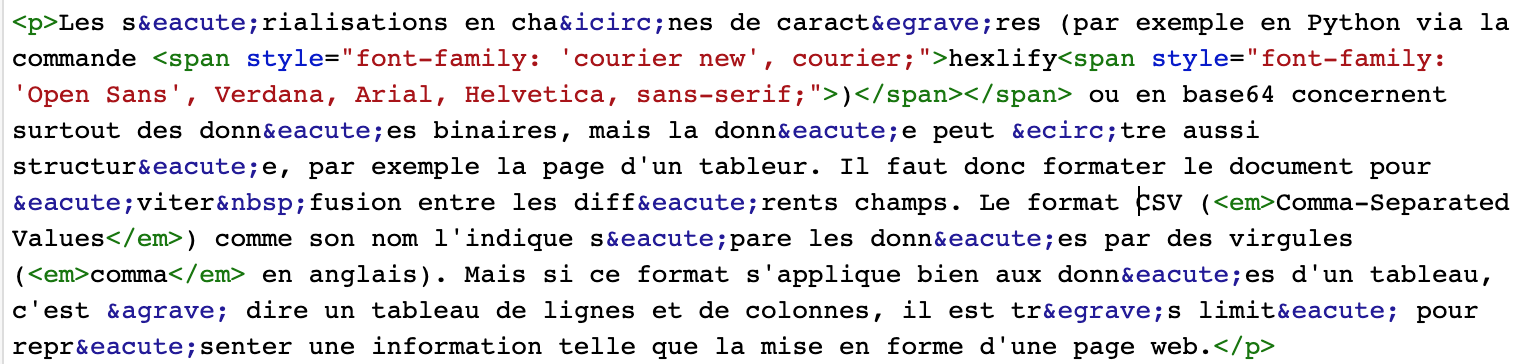
\includegraphics[width=1\columnwidth]{Pictures/Capture22.png}}
\caption{Codage HTML d'une page Web}
\label{fig-HTML}
\end{figure}

Les balises peuvent aussi prendre des arguments, comme la balise \Index{span} dans l'exemple précédent. Ainsi, si l'on regarde une page Web, comme indiqué figure~\vref{fig-Web-HTML}, le navigateur est capable de l'analyser pour trouver les \ac{URI} qu'elle contient. La balise \texttt{\Index{img}} indiquant qu'il s'agit d'une image, le client peut interroger le serveur pour l'afficher à l'écran. Ce format structuré de sérialisation nous permet de mettre en place une caractéristique de \ac{REST}, c'est-à-dire les liens entre ressources.

\begin{figure}[tbp]
\centerline{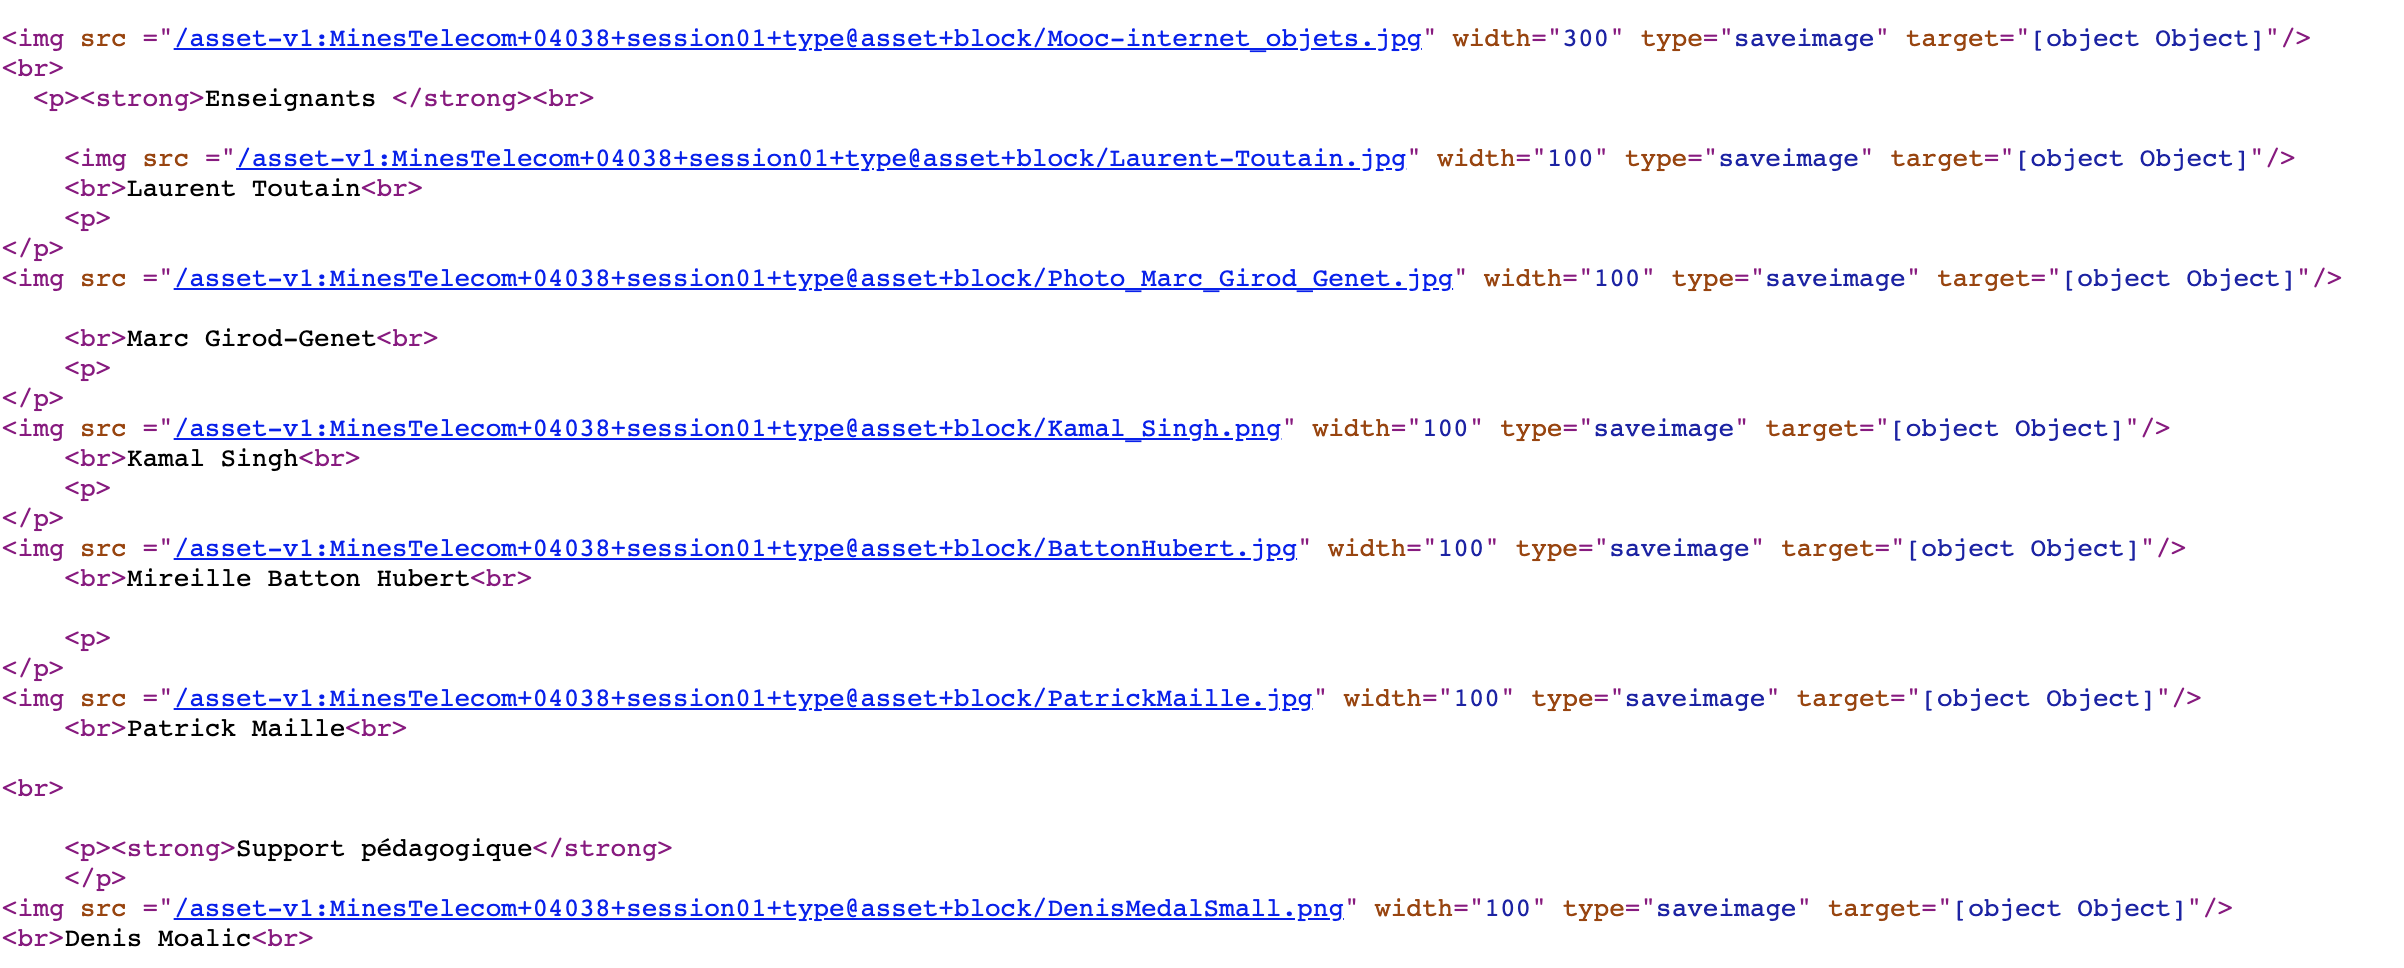
\includegraphics[width=1\columnwidth]{Pictures/Capture23.png}}
\caption{Capture d'une page Web}
\label{fig-Web-HTML}
\end{figure}


\section{XML}

Si \ac{HTML} est dédié au formatage à l'écran de données textuelles et à la navigation sur le Web. \ac{XML}\footnote{\url{https://www.w3.org/TR/xml/}} défini par le \ac{W3C}, est un format d’échange entre deux applications. Par exemple, pour échanger les notes des étudiants entre la plate-forme FUN et une autorité de certification des cours, on pourrait utiliser le format suivant~:

\begin{termc}[backgroundcolor=\color{palerod}]
<etudiant>
   <prenom>John</prenom>
   <nom>Deuf</nom>
   <note>18</note>
</etudiant>

\end{termc}

Il est facile en lisant l'exemple de trouver le prénom, le nom et la note de l'étudiant. On peut noter qu'il n'y a pas de différence entre la note et le nom de l'élève. Il s'agit de caractères.

     \vspace{1em}

S'il est syntaxiquement correct, rien ne dit que le créateur fournit quelque chose de correct qui pourra être interprété par une autre instance.  \ac{XML} peut inclure une grammaire ou un schéma qui est utilisé pour valider que les informations représentées dans le fichier sont non seulement syntaxiquement conformes au langage \ac{XML}, mais aussi conformes au schéma. Ce schéma va décrire les champs attendus et leur type (texte, nombre...). Vous pouvez accéder à ce cours si vous voulez en savoir plus sur les schémas \ac{XML}.

Du point de vue de l’internet des objets, même si le XML pourrait être un bon candidat pour l’échange d’informations, il est un format trop lourd et donc énergivore. On peut noter que pour envoyer une note sur 20 qui, dans l'absolu, prendrait 6 bits, on transmet \texttt{<note>18</note>}, soit 15 caractères soit 120 bits! 

\section{JSON}

 \begin{wrapfigure}{r}{3cm}
\Youtube{https://youtu.be/IhZ9w6jWnq8}
\end{wrapfigure}

\ac{JSON}  offre un moyen de structurer l’information de manière plus compacte que \ac{XML}. JSON s’impose comme le langage commun pour échanger les informations. A l’origine, JSON était utilisé par\Index{Javascriptt} pour échanger des informations ; par exemple, pour afficher en temps réel l’évolution des cours de la bourse ou pour afficher des graphiques dynamiques sur l’écran de l’utilisateur.

JSON \rfc{8259} est un format d’échange simple. Il définit 4 types de données :

\begin{itemize}
    \item nombre~: Les nombres sont composés de chiffres et peuvent être positifs, négatifs, entiers ou flottants.
    \item texte~: Le texte est délimité par des guillemets simples ou doubles.
    \item \Index{tableau}~: Les tableaux sont des listes d’éléments séparés par des virgules et entourés de crochets.
    \item \Index{objet}~: L’objet est une liste de paires composées d’une \Index{clé} et d’une valeur. La clé est une chaîne de caractères et la valeur peut être de n’importe quel type. La clé doit être unique à l’intérieur d’un objet, et référence entièrement la valeur qui la suit. Le couple clé - valeur est séparé par le caractère 2 points  \texttt{:}. Les éléments de l’objet sont séparés par des virgules. L'objet est délimité par des accolades.
\end{itemize}

Par exemple, quelques structures \ac{JSON} :

\begin{itemize}
    \item \texttt{[1, -2, 0.3, 4e1]} est un tableau qui contient 4 nombres ;
    \item \texttt{[1, ”2”, ”34”]} est un tableau contenant un nombre et deux chaines de caractères ;
    \item \texttt{[1, [2, 3 , ”4”]]} est un tableau de deux éléments dont le second est également un tableau de 3 éléments ;
    \item \texttt{\{ ”couleur” : [34, 16, 3]\}} est un objet qui contient un élément et la valeur est un tableau ; 
    \item \texttt{\{ ”name” : ”bob”, ”age” : 30\}} est un objet qui contient deux éléments référencés par les chaînes de caractères (ou index)  ”name” et ”age”.
    
    L’ordre dans lequel sont placés les éléments est indifférent. \texttt{\{”age” : 30, ”name” : ”bob”\}} est équivalent au dernier exemple. 

    Cela impose que l’index utilisé pour accéder à une valeur doit être unique dans la structure objet \texttt{\{”name” : ”bob”, ”name” : ”alice”}\} est interdit.
\end{itemize}

     \vspace{1em}

Le listing suivant donne un exemple de structure JSON tirée du \rfc{8259}. Il contient un objet JSON avec une seule clé \texttt{”Image”}. La valeur de cette clé est une autre structure qui contient six éléments. 

\begin{termc}[backgroundcolor=\color{palerod}, language=json]
{
"Image": {
      "Width": 800,
      "Height": 600,
      "Title": "View from 15th Floor",
      "Thumbnail": {   
           "Url": "http://www.example.com/image/481989943",
           "Height": 125,
           "Width": 100
       },
       "Animated" : false,
       "IDs": [11, 943, 234, 38793]
    }
}
\end{termc}

Le balisage par clé est un élément fondamental dans la structure des données. Il est primordial d'être cohérent et d'assurer une concordance entre émetteur et récepteur sur l'intitulé de la clé pour pouvoir récupérer l'information voulue. De la même façon, il faut s'accorder sur les unités de mesure : une interprétation d'une mesure en centimètre alors qu'elle est en pixel peut être désastreux ; c'est un problème d'interopérabilité.
     \vspace{1em}

JSON est facilement exploitable dans d’autres langages. Par exemple en Python, le module JSON peut être utilisé pour convertir une structure JSON qui est une chaîne ASCII en une représentation interne Python. Les tableaux sont convertis en listes et les objets en dictionnaires.

     \vspace{1em}
     \pythonlst{example\_json.py}

Le programme \pprog{example\_json.py}{cbor-example} reprend la structure précédente. La variable \texttt{struct\_python} est une structure Python. On peut voir que les valeurs pour \texttt{"Animated"} et \texttt{"Copyright"} sont les mots clé Python \texttt{False} (avec un F majuscule) et \texttt{None}. Le programme affiche deux fois cette valeur avec la commande standard \texttt{print} puis avec le module \pfunction{pprint}{pprint} pour avoir un affichage plus lisible. On peut remarquer que l'ordre d'affichage des clés est différent. Comme \texttt{"Title"} était défini deux fois, seul le dernier est conservé dans la structure Python.

\begin{termc}[backgroundcolor=\color{palerod}, language=json, basicstyle=\ttfamily\tiny]
{'Image': {'IDs': [17, 2371, 234, 38793], 'Height': 600, 'Animated': False, 'Title': 'Empty picture', 'Thumbnail': 
{'Url': 'http://www.example.com/image/481989943', 'Width': 100, 'Height': 125}, 'Width': 800, 'Copyright': None}}
{'Image': {'Animated': False,
           'Copyright': None,
           'Height': 600,
           'IDs': [17, 2371, 234, 38793],
           'Thumbnail': {'Height': 125,
                         'Url': 'http://www.example.com/image/481989943',
                         'Width': 100},
           'Title': 'Empty picture',
           'Width': 800}}
\end{termc}

Grâce à la fonction \pfunction{json}{dumps} du module \texttt{json}, la variable \texttt{struct\_python} est transformée en JSON. Les mots clé  \texttt{False} et  \texttt{None} sont remplacés par  \texttt{false} et  \texttt{null}. Le programme affiche une chaîne de caractères.

\begin{termc}[backgroundcolor=\color{palerod}, language=json, basicstyle=\ttfamily\tiny]
{"Image": {"IDs": [17, 2371, 234, 38793], "Height": 600, "Animated": false, "Title": "Empty picture", "Thumbnail": 
{"Url": "http://www.example.com/image/481989943", "Width": 100, "Height": 125}, "Width": 800, "Copyright": null}}
\end{termc}

Pour le retransformer, de JSON en variable Python, on utilise la fonction inverse \pfunction{json}{loads} qui traduit une chaîne de caractères en variable Python.

\begin{termc}[backgroundcolor=\color{palerod}, language=json, basicstyle=\ttfamily\tiny]
{'Image': {'Animated': False,
           'Copyright': None,
           'Height': 600,
           'IDs': [17, 2371, 234, 38793],
           'Thumbnail': {'Height': 125,
                         'Url': 'http://www.example.com/image/481989943',
                         'Width': 100},
           'Title': 'Empty picture',
           'Width': 800}}
\end{termc}


Les autres langues de programmation possèdent également leur propre bibliothèque pour effectuer la traduction.

     \vspace{1em}

Par rapport à \ac{XML}, \ac{JSON} est beaucoup plus permissif et manque de formalisme pour décrire la structure. \ac{JSON-LD} défini par le \ac{W3C} renforce l’interopérabilité de JSON en introduisant des clés spécifiques décrivant la structure des données, une référence aux unités, etc. Nous verrons ces concepts dans la suite du cours.

\section{CBOR}

\begin{wrapfigure}{r}{3cm}
\Youtube{https://youtu.be/thSWuJ-1ld0}
\end{wrapfigure}

\ac{JSON} et \ac{CBOR} sont tous les deux des modes de codage de la donnée.

\ac{JSON} introduit une notation très flexible permettant de représenter toutes les structures de données. Le choix de l'\acs{ASCII} rend ce format universel et n'importe quel ordinateur pourra le comprendre. Mais l'utilisation de l'\acs{ASCII} ne permet pas de transmettre de manière optimale l'information sur un réseau. Quand les réseaux ont un débit raisonnable, cela ne pose pas de problème. Quand on en vient à l'internet des objets, il faut prendre en compte la capacité de traitement limité des équipements et la faible taille des messages échangés.

     \vspace{1em}

Ainsi, en ASCII, la valeur \texttt{123} est codée sur 3 octets (un octet par caractère) tandis qu'en binaire elle n'occuperait qu'un seul octet : \texttt{0111 1011}. 

      \vspace{1em}

\ac{CBOR}, défini dans le \rfc{8949}, permet de représenter les structures de \ac{JSON} mais suivant une représentation binaire. Comme nous le verrons par la suite, si \ac{CBOR} est complètement compatible avec \ac{JSON}, il est possible de représenter d'autres types d'information très utiles dans l'Internet des Objets.

La taille de l'information est réduite et le traitement simplifié. Il faut savoir un peu jongler avec la représentation binaire mais cela reste basique.

      \vspace{1em}

CBOR définit 8 types majeurs qui sont représentés par les 3 premiers bits d'une structure CBOR (cf. figure~\vref{fig-cbor-majeur}). Ces types majeurs ont donc des valeurs comprises entre 0 et 7 (\texttt{000} à \texttt{111} en binaire).

\begin{figure}[tbp]
\centerline{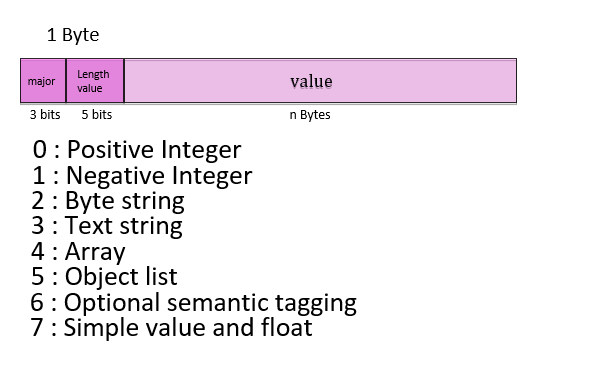
\includegraphics[width=1\columnwidth]{Pictures/cbor1.png}}
\caption{Définition des majeurs en CBOR}
\label{fig-cbor-majeur}
\end{figure}


Les cinq bits suivants contiennent soit une valeur soit une longueur indiquant combien d'octets sont nécessaires pour coder la valeur. \ac{CBOR} offre ainsi des optimisations qui permettent de réduire la longueur totale de la structure des données comme nous le verrons par la suite en étudiant les différents types majeurs.

\subsection{CBOR en python}
Les exemples qui vont suivre peuvent être testés sur votre ordinateur avec Python3. Si une erreur se produit au moment de la définition du module \texttt{\Index{cbor2}}, vous devez l'installer sur votre ordinateur en tapant la commande :

\begin{termc}[backgroundcolor=\color{gray!10}, language=json, basicstyle=\ttfamily\small, escapechar=@]
# @\texttt{pip3 install cbor2}@
\end{termc}


\subsection{Type Entier Positif}
\ac{JSON} ne fait pas de différence entre les nombres, entiers, décimaux, positifs ou négatifs. \ac{CBOR} réintroduit une distinction pour optimiser la représentation.

      \vspace{1em}

Le premier type majeur correspond aux entiers positifs. Il est codé par 3 bits à 0 ; les 5 bits suivants finissent l'octet et, suivant leur valeur, vont avoir une signification différente :
\begin{itemize}
    \item de 0 à 23, il s'agit de la valeur de l'entier à coder ;
    \item 24 indique que l'entier est codé sur 1 octet qui sera codé dans l'octet suivant ;
    \item 25 indique que l'entier est codé sur 2 octets qui seront codés dans les deux octets suivants ;
    \item 26 indique que l'entier est codé sur 4 octets qui seront codés dans les quatre octets suivants ;
    \item 27 indique que l'entier est codé sur 8 octets qui seront codés dans les huit octets suivants.
\end{itemize}

      \vspace{1em}

On peut noter qu'il n'y a pas de surcoût pour coder un entier de 0 à 23. Ainsi, la valeur 15 sera codée 0x0F (\texttt{000-0 1111}) tandis que, pour toutes les autres valeurs supérieures, le surcoût ne sera que d'un octet. La valeur 100 sera codé \texttt{000-1 1000}\footnote{\texttt{11000} correspond à 24} suivi du codage sut 1 octet de la valeur 100 (\texttt{0110 0100}).

      \vspace{1em}

\pythonlst{cbor-integer-ex1.py}

Le programme \pprog{cbor-integer-ex1.py}{cbor-example}  affiche les puissances de $10$ entre $10^0$ et $10^{18}$~:

\begin{itemize}
    \item Ligne 1, le programme importe le module \texttt{\Index{cbor2}} et le renomme pour plus de simplicité \texttt{cbor}.
    \ligne 5, la boucle permet d'avoir les multiples de 10 (variable \texttt{v)}. 
    \item ligne 6, le module \texttt{cbor} utilise comme pour JSON la méthode \pfunction{cbor2}{dumps} pour sérialiser une structure interne de Python dans la représentation demandée. À l'inverse, la méthode \pfunction{cbor2}{loads} sera utilisée pour importer une structure CBOR dans une représentation interne.
    \item Ligne 7, le \texttt{print} permet d'aligner les données pour que l'affichage soit plus clair ; entre les accolades, le premier chiffre indique la position dans les arguments de format ; le second, après le \texttt{:}, le nombre de caractères. Par exemple, \textttt{\{1:30\}} indique l'argument \texttt{v} de format affiché sur 30 caractères.
\end{itemize}
 
       \vspace{1em}

Le programme donne le résultat suivant~:

\begin{termc}[backgroundcolor=\color{palerod}, language=json, basicstyle=\ttfamily\small, escapechar=@]
 # @\textbf{python3 cbor-integer-ex1.py}@
  0                              1 01
  1                             10 0a
  2                            100 1864
  3                           1000 1903e8
  4                          10000 192710
  5                         100000 1a000186a0
  6                        1000000 1a000f4240
  7                       10000000 1a00989680
  8                      100000000 1a05f5e100
  9                     1000000000 1a3b9aca00
 10                    10000000000 1b00000002540be400
 11                   100000000000 1b000000174876e800
 12                  1000000000000 1b000000e8d4a51000
 13                 10000000000000 1b000009184e72a000
 14                100000000000000 1b00005af3107a4000
 15               1000000000000000 1b00038d7ea4c68000
 16              10000000000000000 1b002386f26fc10000
 17             100000000000000000 1b016345785d8a0000
 18            1000000000000000000 1b0de0b6b3a7640000
\end{termc}

       \vspace{1em}


On voit facilement que les valeurs 1 et 10 sont codées sur 1 octet ; que 100 est codé sur 2 octets tandis que les valeurs 1 000 et 10 000 sont codées sur 3 octets. Les valeurs entre 100 000 et 1 000 000 000 nécessitent 5 octets et les valeurs suivantes, 9 octets.

       \vspace{1em}


La taille de la représentation s'adapte à la valeur. Ainsi, il n'est pas nécessaire de définir une taille fixe pour coder une donnée.

On peut aussi noter que comme le type majeur est sur 3 bits, ce type peut être reconnu dans une lecture hexadécimale du résultat car la séquence commence toujours par le symbole \texttt{0} ou \textttt{1}..

\subsection{Type Entier Négatif}

Le type majeur entier négatif est à peu près similaire à l'entier positif. Le type majeur est \texttt{001} et le codage de la valeur se fait sur la valeur absolue du nombre à laquelle on retranche 1. Cela évite deux codes différents pour les valeurs 0 et -0.

       \vspace{1em}

Ainsi, pour coder -15, on va coder la valeur 14, ce qui donne en binaire 001-1 1110. Ainsi, -24 peut également être codé sur 1 octet tandis que +24 sera codé sur 2 octets.

\pythonlst{cbor-integer-ex2.py}

Le programme \pprog{cbor-integer-ex2.py}{cbor-example} reprend le même code que le programme précédent, mais la variable \texttt{v} est initialisée avec la valeur -1. Ce programme va traiter les puissances de 10 négatives.

\begin{termc}[backgroundcolor=\color{palerod}, language=json, basicstyle=\ttfamily\small, escapechar=@]
  # @\textbf{python3.5 cbor-integer-ex2.py}@
  0                             -1 20
  1                            -10 29
  2                           -100 3863
  3                          -1000 3903e7
  4                         -10000 39270f
  5                        -100000 3a0001869f
  6                       -1000000 3a000f423f
  7                      -10000000 3a0098967f
  8                     -100000000 3a05f5e0ff
  9                    -1000000000 3a3b9ac9ff
 10                   -10000000000 3b00000002540be3ff
 11                  -100000000000 3b000000174876e7ff
 12                 -1000000000000 3b000000e8d4a50fff
 13                -10000000000000 3b000009184e729fff
 14               -100000000000000 3b00005af3107a3fff
 15              -1000000000000000 3b00038d7ea4c67fff
 16             -10000000000000000 3b002386f26fc0ffff
 17            -100000000000000000 3b016345785d89ffff
 18           -1000000000000000000 3b0de0b6b3a763ffff
\end{termc}


\subsection{Type Séquence binaire ou Chaîne de caractères}

Les séquences binaires et les chaînes de caractères ont le même comportement. Le type majeur est respectivement \texttt{010} et \texttt{011}. Il est suivi par la longueur de la séquence ou de la chaîne. Le même type de codage que pour les entiers est utilisé :
\begin{itemize}
    \item si la longueur est inférieure à 23, elle est codée dans la suite du premier octet. On trouve ensuite le nombre d'octets ou de caractères correspondant à cette longueur ;
    \item si la longueur peut être codée dans 1 octet (donc inférieure à 255), la suite du premier octet contient 24 puis l'octet suivant contient la longueur suivie du nombre d'octets ou de caractères correspondant.
    \item si la longueur peut être codée dans 2 octets (donc inférieure à 65535), la suite du premier octet contient 25 puis l'octet suivant contient la longueur suivie du nombre d'octets ou de caractères correspondant.
    \item si la longueur peut être codée dans 4 octets, la suite du premier octet contient 26 puis l'octet suivant contient la longueur suivie du nombre d'octets ou de caractères correspondant.
    \item si la longueur peut être codée dans 8 octets, la suite du premier octet contient 27 puis l'octet suivant contient la longueur suivie du nombre d'octets ou de caractères correspondant.
\end{itemize}

       \vspace{1em}

Ce codage est aussi assez optimal. Il est rare d'envoyer plus de 23 caractères.

\pythonlst{cbor-string.py}

Le programme \pprog{cbor-string.py}{cbor-example} montre la représentation de chaînes de caractères de longueur croissante ainsi qu'une séquence binaire~:

\begin{itemize}
    \item ligne 3, la variable \texttt{i} prend des valeurs de 1 à 9.
    \item ligne 6, La multiplication d'une chaîne de caractères par un entier (ligne 4) indique le nombre de répétitions de celle-ci.
    \item lignes 8 et 9 montrent le codage d'une chaîne d'octets. La variable bs contient la représentation en CBOR d'une chaîne d'octets Python (représenté par le caractère \texttt{b} avant les guillemets, les valeurs qui ne correspondent pas à des caractères ASCII sont précédées des symboles \texttt{$\backslash$x}). La représentation en hexadécimal de l'objet CBOR est ensuite affichée.
\end{itemize}

       \vspace{1em}

 
Le résultat est le suivant :

\begin{termc}[backgroundcolor=\color{palerod}, language=json, basicstyle=\ttfamily\tiny, escapechar=@]
# @\textbf{python3.5 cbor-string.py}@
  1 674c6f526157414e
  2 6e4c6f526157414e4c6f526157414e
  3 754c6f526157414e4c6f526157414e4c6f526157414e
  4 781c4c6f526157414e4c6f526157414e4c6f526157414e4c6f526157414e
  5 78234c6f526157414e4c6f526157414e4c6f526157414e4c6f526157414e4c6f526157414e
  6 782a4c6f526157414e4c6f526157414e4c6f526157414e4c6f526157414e4c6f526157414e4c6f526157414e
  7 78314c6f526157414e4c6f526157414e4c6f526157414e4c6f526157414e4c6f526157414e4c6f526157414e4c6f526157414e
  8 78384c6f526157414e4c6f526157414e4c6f526157414e4c6f526157414e4c6f526157414e4c6f526157414e4c6f526157414e4c6f526157414e
  9 783f4c6f526157414e4c6f526157414e4c6f526157414e4c6f526157414e4c6f526157414e4c6f526157414e4c6f526157414e4c6f526157...
43010203
\end{termc}


Jusqu'à 3 répétitions de la chaîne de caractères "LoRaWAN", le codage de la longueur est optimal (codé sur 2 octets).

\subsection{Type tableau}

Le type tableau va regrouper un ensemble d'éléments. Chacun de ces éléments étant une structure CBOR, la seule information nécessaire pour connaître le début et la fin d'un tableau est son nombre d'éléments. Le type majeur est \texttt{100}. Il existe deux méthodes pour coder la longueur d'un tableau :
\begin{itemize}
    \item si celle-ci est connue au moment du codage, il suffit de l'indiquer avec un codage identique à celui utilisé pour indiquer la longueur d'une chaîne de caractères ;
    \item si celle-ci n'est pas connue au moment du codage, il existe un code spécial pour indiquer la fin du tableau. Nous en reparlerons par la suite.
\end{itemize}

\pythonlst{cbor-array.py}

Le programme \pprog{cbor-array.py}{cbor-example} donne quelques exemples de codage de tableau :
\begin{itemize}
    \item \texttt{[1,2,3,4]} défini ligne 3, devient \texttt{8401020304}. On peut deviner la structure du message CBOR : \texttt{0x84} indique un tableau de 4 éléments (attention le décodage n'est pas toujours aussi simple). Les 4 éléments sont des entiers inférieurs à 23 ;
    \item \texttt{[1,[2, 3], 4]} défini ligne 7 devient \texttt{8301\ul{820203}04}. Il s'agit d'un tableau de 3 éléments dont le deuxième est un tableau de deux éléments ;
    \item \texttt{[1000, +20, -10, +100, -30, -50, 12]} défini ligne 11, devient \texttt{871903e814291864 381d38310c}. On peut noter que le codage des éléments est de longueur variable, mais comme chaque élément code sa longueur, il est juste nécessaire d'en connaître le nombre.
\end{itemize}

\subsection{Type map (Liste de paires)}



Le type Liste de paires ou Map est indiqué par la valeur \texttt{101}. Il fonctionne de la même manière que les tableaux en comptant le nombre d'éléments. Mais cette fois-ci, la valeur représente une paire, c'est-à-dire deux objets CBOR consécutifs.

\pythonlst{cbor-mapped.py}

Le programme \pprog{cbor-mapped.py}{cbor-example} donne un exemple d'encodage. A noter que la structure à encoder n'est pas directement compatible avec JSON\footnote{json.\pfunction{json}{dumps} aurait converti les clés numériques en chaînes de caractères \texttt{'\{"type": "hamster", "2": "program", "taille": 300, "15": 113\}'}}, certaines clés ne sont pas des chaînes de caractères.

       \vspace{1em}


Le résultat est \texttt{a464747970656768616d73746572667461696c6c6519012c026770726f6772 616d0f1871} ce qui n'est pas très facile à lire. 


\subsubsection{cbor.me}

\begin{wrapfigure}{r}{3cm}
\Youtube{https://youtu.be/h1XnaFy_FoI}
\end{wrapfigure}

Le site web \url{https://cbor.me} permet de faire automatiquement le codage dans un sens ou dans l'autre.
La colonne de gauche représente la donnée en JSON et celle de droite en CBOR (dite "représentation canonique" qui facilite la lecture). En ayant entré la séquence hexadécimale ci-dessus, le site la présente comme indiqué figure~\vref{fig-cbor-me}.
La partie CBOR est indexée et commentée pour rendre l'objet CBOR plus lisible. Il peut également être traduit dans un équivalent JSON, bien que certaines clés restent numériques.

\begin{figure}[tbp]
\centerline{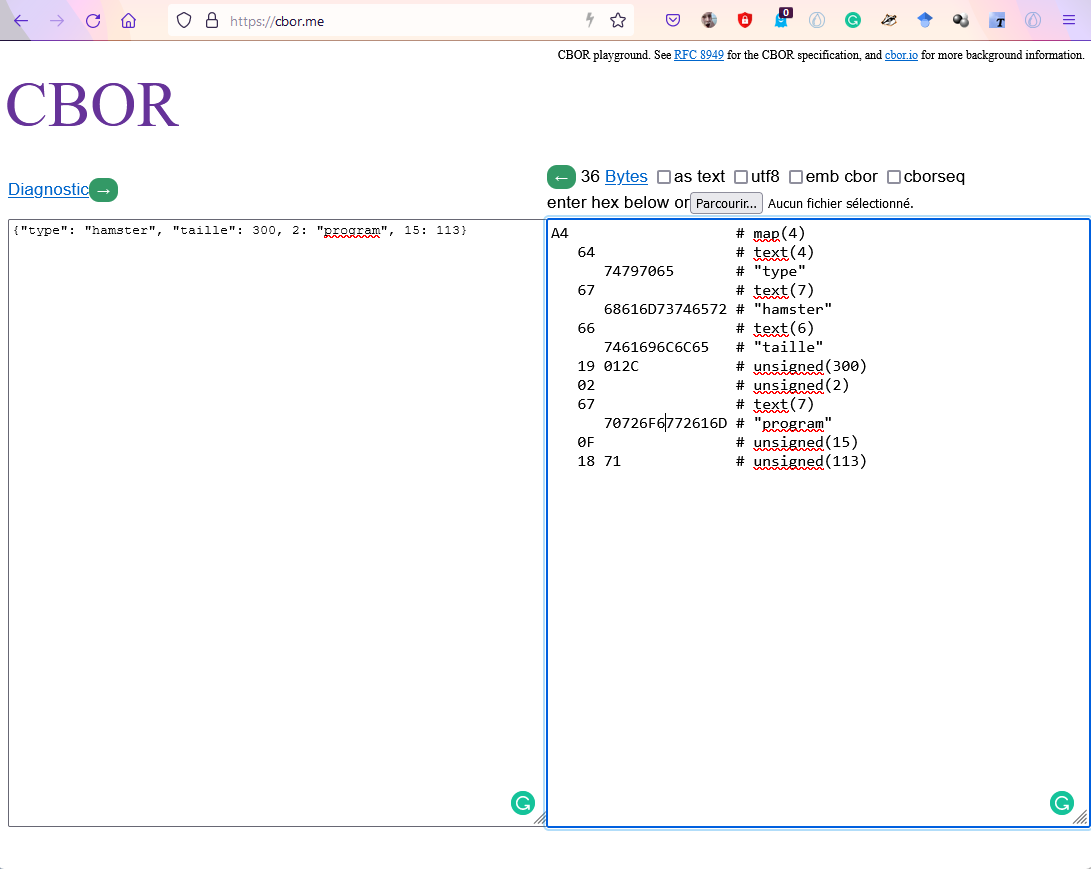
\includegraphics[width=1\columnwidth]{Pictures/cbor-me.png}}
\caption{Définition des majeurs en CBOR}
\label{fig-cbor-me}
\end{figure}

Sur ces exemples, on peut voir que CBOR est beaucoup plus permissif et complet que JSON, le premier champ des map CBOR peut être numérique et n'a pas à être unique dans toute la structure. Néanmoins  CBOR
définit un mode strict dans lequel ces clés doivent être codées en ASCII et unique pour être compatibles avec
JSON. Si une clé est répété plusieurs fois dans une structure CBOR, il traiter directement l'information dans la structure CBOR et ne pas chercher à la convertir ou la désérialiser car il y a un risque de perte d'information. 

\subsection{Type étiquette}

CBOR enrichit le typage des données ; ce qui permet de manipuler plus facilement des données. Par exemple, une chaîne de caractères peut représenter une date, une URI, voire une URI codée en base 64. Le type \texttt{110} peut être suivi d'une valeur ou \Index{tag} dont une liste exhaustive est maintenue parl'IANA\footnote{\url{https://www.iana.org/assignments/cbor-tags/cbor-tags.xhtml}}.

\pythonlst{cbor-tag.py}

Par exemple, le programme \pprog{cbor-tag.py}{cbor-example} retourne les résultats suivants:

\begin{termc}[backgroundcolor=\color{palerod}, language=json, basicstyle=\ttfamily\small, escapechar=@]
# @\textbf{python3.5 cbor-tag.py}@
2018-05-22
c074323031382d30352d32325430303a30303a30305a
2018-05-22 00:00:00+00:00
43010203
<class 'datetime.datetime'>
\end{termc}


La représentation canonique montre plus facilement le tag dans la séquence binaire :
\begin{termc}[backgroundcolor=\color{palerod}, language=json, basicstyle=\ttfamily\small, escapechar=@]
C0                                      # tag(0)
   74                                   # text(20)
      323031382D30352D32325430303A30303A30305A # "2018-05-22T00:00:00Z"
\end{termc}

Le tag 0 implique un format normalisé pour la date ; d'où l'ajout des heures, minutes et secondes, alors qu'elles n'ont pas été spécifiées initialement. On peut également remarquer que \pfunction{cbor2}{loads} retourne un type \texttt{date} et non une chaîne de caractères.

\subsection{Le type flottant et valeurs particulières}
Le dernier type majeur (111) permet de coder les nombres flottants en utilisant la représentation définie par l'\Index{IEEE 754}. Suivant la taille de la représentation, la suite de l'octet contient les valeurs 25 (demi précision sur 16 bits), 26 (simple précision sur 32 bits) ou 27 (double précision sur 64 bits).

Ce type permet également de coder les valeurs définies par JSON : True (valeur 20), False (valeur 21) ou None (valeur 22).

Finalement, ce type peut indiquer la fin d'un tableau ou d'une liste de paires quand la taille n'est pas connue au début du codage.

\section{Questions sur CBOR}
\Question{Avantages de CBOR}{
Quel sont les avantage de CBOR par rapport à JSON (2 réponses) ?
\begin{itemize}[label=$\square$]
   \item \Correct{Il est plus compact dans la représentation des données.}
   \item \Wrong{Il permet de représenter des nombres flottants.}
   \item \Wrong{Il compresse les chaînes de caractères. }
   \item \Correct{Il est plus simple à implémenter.}
 \end{itemize}
   
 }
{
CBOR ne compresse pas les chaînes de caractères. Il ajoute juste leur longueur. CBOR et JSON codent tous les deux des nombres flottants, ce n'est donc pas un avantage de CBOR. Par contre, le fait d'utiliser des valeurs binaires au lieu de l'ASCII pour représenter les nombres, de ne pas avoir de crochets ou accolades, permet d'avoir une représentation beaucoup plus compacte. Les petites valeurs numériques sont représentées sans surcoût. Réaliser un codeur ou un décodeur de CBOR est beaucoup plus simple qu'en JSON car la représentation des données est beaucoup plus stricte (pas d'espace, pas de retour à la ligne... ). Les deux représentations permettent d'utiliser des nombres flottant donc aucune n'a d'avantage sur ce point.
}

\Question{Flottant}{
Un flottant est-il toujours plus compact en CBOR qu'en JSON ? - Vous pouvez vous aider de \url{https://cbor.me}

\begin{itemize}[label=$\circ$]
   \item \Wrong{Oui, c'est le but de CBOR.}
   \item \Wrong{Oui pour les flottants qui ont la partie décimale à 0..}
   \item \Wrong{Oui pour les flottants de petite précision (jusqu'au centième).}
   \item \Correct{Oui pour les flottants de grande précision (6 chiffres après la virgule).}
 \end{itemize}
}{
Un nombre flottant, quelle que soit sa valeur, est représenté par 8 octets en CBOR. En JSON, un nombre flottant est représenté par une chaîne de caractères. Donc "3.0" nécessite 3 caractères, donc plus compacte que CBOR. Mais "3.1415926" est codé sur 9 caractères donc moins compacte que CBOR.
}

\Question{Chaîne de caractères}{
Soit une chaîne de caractères en CBOR.
\begin{itemize}[label=$\circ$]
   \item \Wrong{Elle est compressée avec un algorithme entropique (e.g. codage de Huffman).}
   \item \Correct{Elle peut contenir des caractères accentués.}
   \item \Wrong{Chaque caractère est codé sur 6 bits.}
 \end{itemize}

}{
Une chaîne de caractères est une séquence d'octets. Il est possible d'utiliser les représentations offrant des caractères accentués (voire des émoticones). Par contre, CBOR ne compresse pas les données.
}

\Question{Taille variable}{
-En CBOR, la taille d'un entier varie en fonction de sa valeur !
\begin{itemize}[label=$\circ$]
   \item \Correct{Vrai}
   \item \Wrong{Faux}
   \item \Wrong{Ça dépend de la manière dont on a déclaré cet entier.}
 \end{itemize}

}{
Oui, un entier inférieur à 23 sera codé sur un seul octet. Pour les valeurs plus grandes, il faut ajouter la longueur.
}

\Question{Tableau}{
En CBOR, un tableau peut contenir des objets de types différents.
\begin{itemize}[label=$\circ$]
   \item \Correct{Vrai}
   \item \Wrong{Faux}
   \item \Wrong{Ça dépend de la manière dont on a déclaré ce tableau.}
 \end{itemize}
}{
Vrai, on a la même flexibilité qu'en JSON en imbriquant n'importe quel type de données dans un tableau.
}

\Question{Fraction}{
On veut définir un tableau de deux éléments comme une fraction. Quel tag devra précéder la structure ?
(vous pouvez vous aider du \rfc{8949}.
}{
Il s'agit du tag 4, voir le chapitre \textbf{3.4.4. Decimal Fractions and Bigfloats} du \rfc{8949}.
}

\section{SenML}

\ac{SenML} est une une spécification qui exploite JSON ou CBOR. Elle liste un ensemble de noms/unités/mesures et les standardise en un nom de clé unique. En utilisant cette standardisation, on facilite l'interopérabilité. Les clés et valeurs sont donc règlementées et typées pour éviter tous conflits d'interopérabilité. Le format est défini dans la \rfc{8428} et repose sur une structure de tableau regroupant des objets comme le montre la figure suivante tirée de la RFC.

\begin{termc}[backgroundcolor=\color{palerod}, language=json, basicstyle=\ttfamily\small, escapechar=@]
[
 {"bn" : "urn:dev:ow:10e2073a01080063", "bt":1.320067464e+09,
  "bu" : "\%RH", "v":21.2},
 {"t":10, "v":21.3},
 {"t":20, "v":21.4},
 {"t":30, "v":21.4},
...
\end{termc}

SenML définit les clés utilisées dans l’objet. Pour avoir une notation compacte, elles sont limitées à 1 ou 2 caractères. Parmi elles, ”bn” indique un nom de base et ”n” le nom d’un appareil. Si plusieurs appareils envoient la partie commune de l’identifiant de l’appareil, on peut mettre le ”bn” pour éviter de le répéter à chaque fois.

Le temps de base (ou ”bt”) est également un moyen de compacter la notation du temps. Le temps (”t”) donne le décalage et conduit à une valeur plus petite comme on le voit dans l’exemple.

L’unité de base (”bu”) indique l’unité par défaut si les autres objets ne portent pas de mot clé indiquant l’unité (”u”).

La \rfc{8428} définit une liste d’unités telles que le kilogramme (”kg”), le volt (”V”), etc. Dans l’exemple, ”%RH” désigne un pourcentage d’humidité relative. Une valeur numérique utilise la lettre ”v”, une chaîne de caractères utilise la touche ”vs”.

CBOR utilise la même structure mais les petits nombres entiers positifs et négatifs sont substitués dans les clés des objets de CBOR : ”bn”, ”bt”, ”bu” seront respectivement représentés par -1, -2 et -3 et ”n”, ”t”, ”u” par +0, +2 et +6.


